\documentclass{article}
\usepackage[a4paper,margin=1in,footskip=0.25in]{geometry}
\usepackage{listings}
\usepackage{hyperref}
\hypersetup{
	 colorlinks   = true,
     citecolor    = black,
     linkcolor    = black,
     urlcolor     = black
}
\usepackage{graphicx}
\usepackage{algorithm}
\usepackage{algpseudocode}
\usepackage{amsmath}
\usepackage{tikz}
\usepackage{caption}
\usepackage{subcaption}
\usepackage{float}
\usetikzlibrary{arrows,matrix,positioning}
\setcounter{tocdepth}{3}

\begin{document}
\title{DIP Homework 2}
\author{Qiuyi Zhang 12330402 \\ \href{mailto:joyeec9h3@gmail.com}{joyeec9h3@gmail.com}} 
\date{\today}
\maketitle
\tableofcontents
\section{Exercises}

\subsection{Histogram Equalization}

\textbf{Answer:} 
Let $MN$ be the total number of pixels, $n_{r_j}$ be the number of pixels in the original image with intensity value $r_j$, $L$ be the intensity levels of the image. From eq. (3.3-8) in the textbook, the histogram equalization transformation would be:

$$s_k = \frac{(L-1)}{MN}\sum_{r_j=0}^{r_k}n_{r_j}$$

Hence $s_k$ is monotonically increasing, therefore $n_{s_k} = n_{r_k}$. The second pass of histogram equalization would produce:

$$v_k =  \frac{(L-1)}{MN}\sum_{s_j=0}^{s_k}n_{s_j}$$

Because $n_{s_k} = n_{r_k}$, 

$$v_k =  \frac{(L-1)}{MN}\sum_{r_j=0}^{r_k}n_{r_j} = s_k$$

This shows that a second pass of histogram equalization produces exactly the same result as the first pass.

\subsection{Spatial Filtering}

\textbf{Answer:}
The merging of the bars in Fig. 1(c) is caused by the width of the filter matching the width of a bar plus the distance between the bars. When the filter is shifted between the bars, it will always cover exactly the same group of pixels that make up one bar, so the numerator for the averaging operator will always be the same within this area. Because the denominator is a constant for a given averaging filter, it will produce the same response across the area containing the bars, therefore the bars seem to be merged. But in Fig. 1(b) and Fig. 1(d), the width of the filter is smaller/larger than, or not a multiple of, the width of a bar plus the distance between the bars. Therefore there are no merging effects in these two figures.

% -------------------- Programming Tasks ------------------------
\section{Programming Tasks}
% -------------------- Histogram Equalization ------------------------
\subsection{Histogram Equalization}
% -------------------- Results ------------------------
\subsubsection{Results}
\begin{figure}[H]
	\centering
	% pt = px * 72 / DPI
	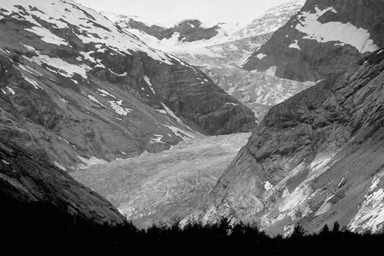
\includegraphics[width=288pt]{../img/02.png}
	\caption{The original image}
\end{figure}

\begin{figure}[H]
	\centering
	% pt = px * 72 / DPI
	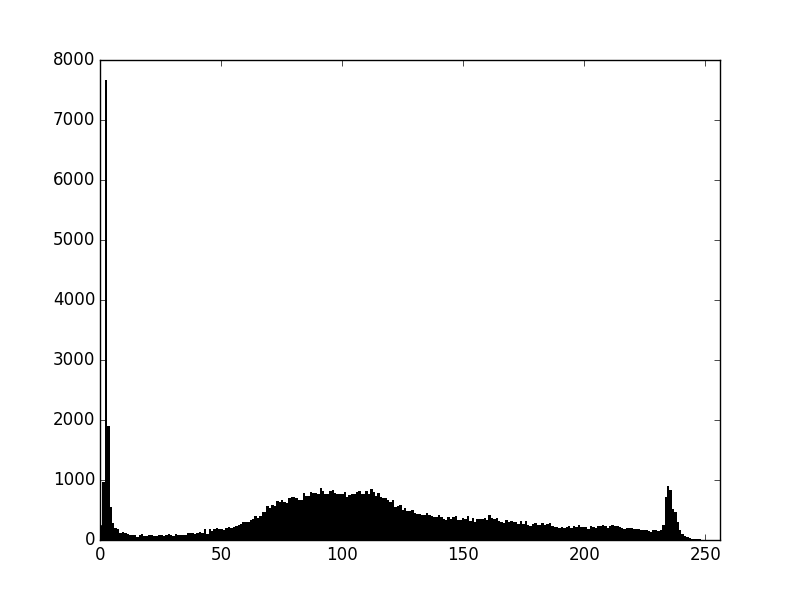
\includegraphics[width=300pt]{../result/hist.png}
	\caption{Histogram of the original image}
\end{figure}

\begin{figure}[H]
	\centering
	% pt = px * 72 / DPI
	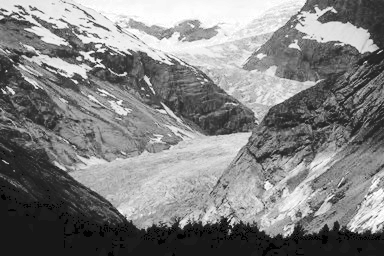
\includegraphics[width=288pt]{../result/equalize.png}
	\caption{Histogram-equalized result}
\end{figure}

\begin{figure}[H]
	\centering
	% pt = px * 72 / DPI
	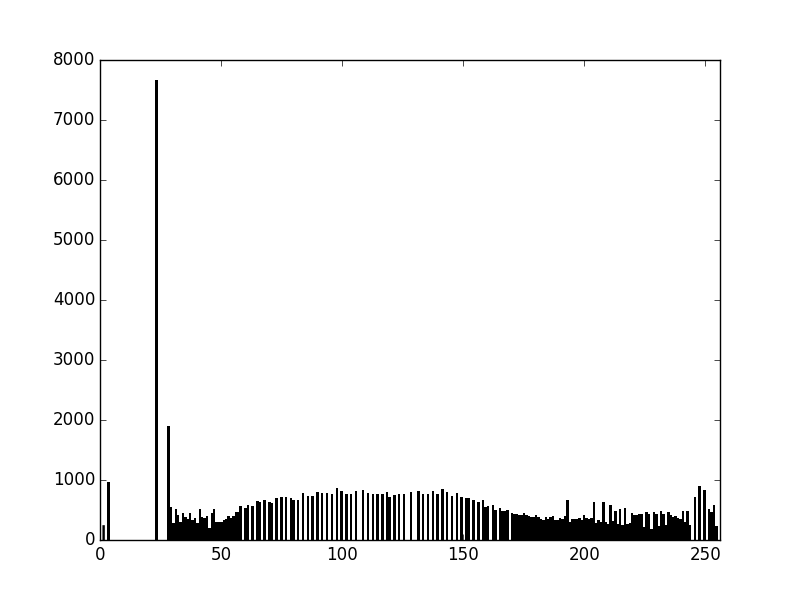
\includegraphics[width=300pt]{../result/hist-equalize.png}
	\caption{Histogram of the histogram-equalized result}
\end{figure}

% -------------------- Discussion ------------------------
\subsubsection{Analysis}

\paragraph{}
After histogram equalization, the image covers a wider range of intensity scale, therefore the result has a higher contrast. The snow on the mountain is whiter and the shades has more layers after being processed.

The equalized histogram clearly has a more uniformed plot, though inevitably there are some extreme values that still stand out after equalization, like the dark regions at the bottom of the image which results in the high bars in the left of the plot.

% -------------------- Algorithm ------------------------
\subsubsection{Algorithm}

\begin{algorithm}[H]
\centering
\caption{Histogram Equalization}
  \begin{algorithmic}[1]
    \Function{equalize\_hist}{$input\_img$}
     \State $L = $ intensity levels of the $input\_img$
     \State $MN = $ number of pixels in $input\_img$
      \For{$i = 0 \to L - 1$}
      	\State $n_i = $ number of pixels in $input\_img$ with intensity level $i$
      	\State $s_i = 0$
      	\For{$j = 0 \to i$}
      		\State $s_i += n_j$
      	\EndFor
      	\State $s_i = s_i \times \frac{(L - 1)}{MN}$
      \EndFor
      \For{each pixel $p$ in $input\_img$}
      	\State $i = $ the intensity of $p$
      	\State Put a pixel with intensity $s_i$ into $output\_img$
      \EndFor
      \State \Return $output\_img$
    \EndFunction
  \end{algorithmic}
\end{algorithm}

% -------------------- Image Patch Extraction ------------------------

\subsection{Image Patch Extraction}

% -------------------- Results ------------------------
\subsubsection{Results}
\begin{figure}[H]
	\centering
	% pt = px * 72 / DPI
	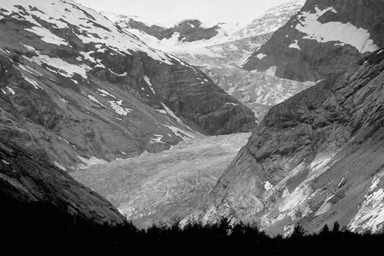
\includegraphics[width=288pt]{../img/02.png}
	\caption{The original image}
\end{figure}

\begin{figure}[H]
	\begin{minipage}[b]{0.24\linewidth}
		\centering
		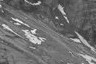
\includegraphics[width=72pt]{../result/patch-96-64-0.png}
	\end{minipage}
	\begin{minipage}[b]{0.24\linewidth}
		\centering
		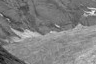
\includegraphics[width=72pt]{../result/patch-96-64-1.png}
	\end{minipage}
	\begin{minipage}[b]{0.24\linewidth}
		\centering
		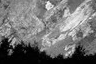
\includegraphics[width=72pt]{../result/patch-96-64-2.png}
	\end{minipage}
	\begin{minipage}[b]{0.24\linewidth}
		\centering
		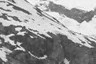
\includegraphics[width=72pt]{../result/patch-96-64-3.png}
	\end{minipage}
\end{figure}

\begin{figure}[H]
	\begin{minipage}[b]{0.24\linewidth}
		\centering
		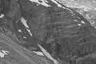
\includegraphics[width=72pt]{../result/patch-96-64-4.png}
	\end{minipage}
	\begin{minipage}[b]{0.24\linewidth}
		\centering
		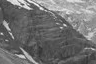
\includegraphics[width=72pt]{../result/patch-96-64-5.png}
	\end{minipage}
	\begin{minipage}[b]{0.24\linewidth}
		\centering
		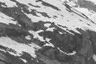
\includegraphics[width=72pt]{../result/patch-96-64-6.png}
	\end{minipage}
	\begin{minipage}[b]{0.24\linewidth}
		\centering
		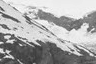
\includegraphics[width=72pt]{../result/patch-96-64-7.png}
	\end{minipage}
	\caption{96 $\times$ 64 patches}
\end{figure}

\begin{figure}[H]
	\begin{minipage}[b]{0.24\linewidth}
		\centering
		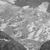
\includegraphics[width=37.5pt]{../result/patch-50-50-0.png}
	\end{minipage}
	\begin{minipage}[b]{0.24\linewidth}
		\centering
		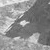
\includegraphics[width=37.5pt]{../result/patch-50-50-1.png}
	\end{minipage}
	\begin{minipage}[b]{0.24\linewidth}
		\centering
		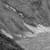
\includegraphics[width=37.5pt]{../result/patch-50-50-2.png}
	\end{minipage}
	\begin{minipage}[b]{0.24\linewidth}
		\centering
		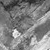
\includegraphics[width=37.5pt]{../result/patch-50-50-3.png}
	\end{minipage}
\end{figure}

\begin{figure}[H]
	\begin{minipage}[b]{0.24\linewidth}
		\centering
		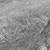
\includegraphics[width=37.5pt]{../result/patch-50-50-4.png}
	\end{minipage}
	\begin{minipage}[b]{0.24\linewidth}
		\centering
		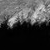
\includegraphics[width=37.5pt]{../result/patch-50-50-5.png}
	\end{minipage}
	\begin{minipage}[b]{0.24\linewidth}
		\centering
		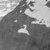
\includegraphics[width=37.5pt]{../result/patch-50-50-6.png}
	\end{minipage}
	\begin{minipage}[b]{0.24\linewidth}
		\centering
		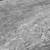
\includegraphics[width=37.5pt]{../result/patch-50-50-7.png}
	\end{minipage}
	\caption{50 $\times$ 50 patches}
\end{figure}

% -------------------- Spatial Filtering ------------------------
\subsection{Spatial Filtering}

% -------------------- Results ------------------------
\subsubsection{Results}

\begin{figure}[H]
	\centering
	% pt = px * 72 / DPI
	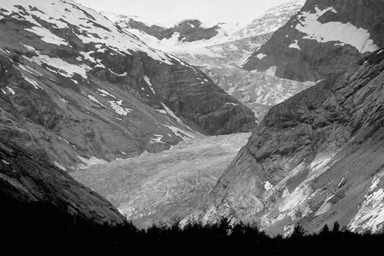
\includegraphics[width=288pt]{../img/02.png}
	\caption{The original image}
\end{figure}

\begin{figure}[H]
	\centering
	% pt = px * 72 / DPI
	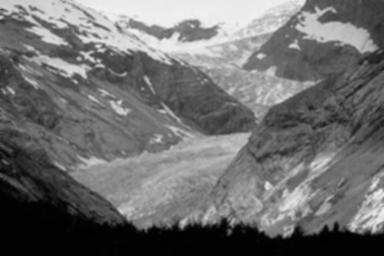
\includegraphics[width=288pt]{../result/filter-smooth-3-3.png}
	\caption{Smoothed image with $3 \times 3$ averaging filter}
\end{figure}

\begin{figure}[H]
	\centering
	% pt = px * 72 / DPI
	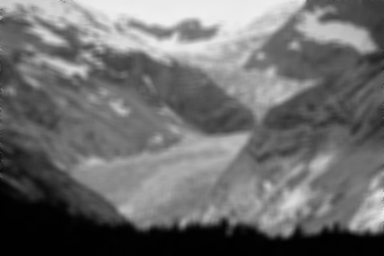
\includegraphics[width=288pt]{../result/filter-smooth-7-7.png}
	\caption{Smoothed image with $7 \times 7$ averaging filter}
\end{figure}

\begin{figure}[H]
	\centering
	% pt = px * 72 / DPI
	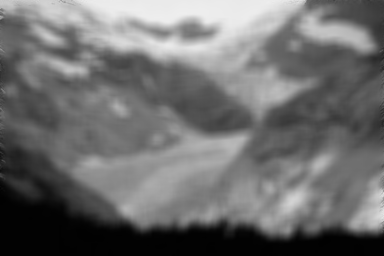
\includegraphics[width=288pt]{../result/filter-smooth-11-11.png}
	\caption{Smoothed image with $11 \times 11$ averaging filter}
\end{figure}

\begin{figure}[H]
	\centering
	% pt = px * 72 / DPI
	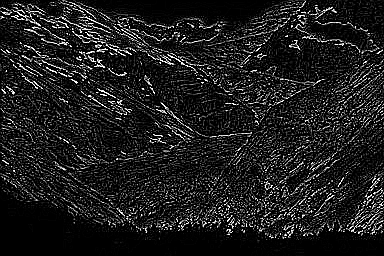
\includegraphics[width=288pt]{../result/filter-laplacian.png}
	\caption{Image filtered with $3 \times 3$ Laplacian filter}
\end{figure}

\begin{figure}[H]
	\centering
		\[ \begin{bmatrix}
			-1 & -1 & -1 \\
			-1 &  8 & -1 \\
			-1 & -1 & -1
		\end{bmatrix} \]
\caption{Laplacian filter}
\end{figure}

\begin{description}
\item[Note] \hfill \\
To obtain a sharpened image with the result of a laplacian filter, we can combine the original image with the filtered result. Because the laplacian filter used here has a positive center, the sharpened image can be produced by:

$$g(x,y) = f(x, y) + laplacian(x, y)$$

where $g(x, y)$, $f(x, y)$, and $laplacian(x, y)$ are intensity values at the pixels of coordinate $(x, y)$ in the sharpened image, original image, and the laplacian filtered image, respectively.
\end{description}

\begin{figure}[H]
	\centering
	% pt = px * 72 / DPI
	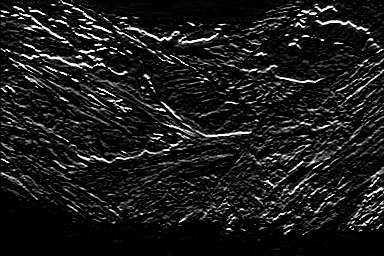
\includegraphics[width=288pt]{../result/filter-sobel-0.png}
	\caption{Image filtered with $3 \times 3$ horizontal Sobel filter}
\end{figure}

\begin{figure}[H]
	\centering
	% pt = px * 72 / DPI
	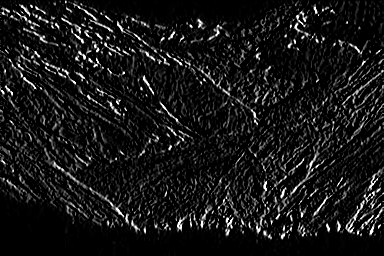
\includegraphics[width=288pt]{../result/filter-sobel-1.png}
	\caption{Image filtered with $3 \times 3$ vertical Sobel filter}
\end{figure}

\begin{figure}[H]
	\centering
	\begin{minipage}[b]{0.30\linewidth}
		\[ \begin{bmatrix}
			-1 & -2 & -1 \\
			 0 &  0 &  0 \\
			 1 &  2 &  1
		\end{bmatrix} \]
		\subcaption{$3 \times 3$ horizontal Sobel filter}
	\end{minipage}
	\begin{minipage}[b]{0.30\linewidth}
		\[ \begin{bmatrix}
			-1 &  0 &  1 \\
		    -2 &  0 &  2 \\
			-1 &  0 &  1
		\end{bmatrix} \]
		\subcaption{$3 \times 3$ vertical Sobel filter}
	\end{minipage}
	\caption{Sobel filters}
\end{figure}

\begin{description}
\item[Note] \hfill \\
The two filtered result contain the vertical and horizontal derivatives of the original image respectively. To obtain the magnitude of gradient from these two partial derivatives, we can calculate the square root of the sum of the squares:

$$M(x,y) = \sqrt{g_{x}(x, y)^2 + g_{y}(x, y)^2}$$

or approximate the value by calculating:

$$M(x,y) \approx |g_{x}(x, y)| + |g_{y}(x, y)|$$

where $M(x, y)$, $g_{x}(x, y)$, and $g_{y}(x, y)$ are intensity values at the pixels of coordinate $(x, y)$ in the gradient image, horizontally filtered image, and the vertically filtered image, respectively.

To obtain a sharpened image with the gradient, we can calculate:

$$g(x,y) = f(x, y) + M(x, y)$$

where $g(x, y)$, $f(x, y)$, and $M(x, y)$ are intensity values at the pixels of coordinate $(x, y)$ in the sharpened image, original image, and the gradient image, respectively.

\end{description}

% ---------------------- Discussion ---------------------------
\subsubsection{Applications of different filters}

\begin{description}
\item[Averaging filter] \hfill
\begin{itemize}
\item Smooth or blur the image.
\item Reduce noise.
\item Combined with thresholding function to obtain a gross representation of an image.
\end{itemize}
\item[Median filter] \hfill
\begin{itemize}
\item Smooth or blur the image.
\item Reduce noise, especially \textit{salt-and-pepper} noise.
\end{itemize}
\item[Max filter] \hfill
\begin{itemize}
\item Find the brightest points in an image.
\end{itemize}
\item[Min filter] \hfill
\begin{itemize}
\item Find the darkest points in an image.
\end{itemize}
\item[Laplacian filter] \hfill
\begin{itemize}
\item Detect edges, corners, features, blobs in an image.
\item Estimate motions in images.
\end{itemize}
\item[Sobel filter] \hfill
\begin{itemize}
\item Detect edges, corners, features, blobs in an image.
\end{itemize}
\end{description}

% ---------------------- Algorithm ---------------------------
\subsubsection{Algorithm}

\begin{description}
\item[Note] \hfill \\
The textbook uses zero padding for the example of correlation, but it also mentions that duplicates or mirror values can be used for padding (see side notes on P169). Here I use the duplicate of the neighborhood center for padding when dealing with borders because it produces a more natural result.

\end{description}

\begin{algorithm}[H]
\centering
\caption{Filter}
  \begin{algorithmic}[1]
    \Function{filter2d}{$input\_img, filter$}
     \State $N = $ width of $input\_img$, $M = $ height of $input\_img$
     \State $n = $ width of $filter$, $m = $ height of $filter$
     \State $a = \lfloor{\frac{m}{2}}\rfloor$, $b = \lfloor{\frac{n}{2}}\rfloor$
     \State $w$ = the $filter$ flattened to 1-d
     \For{each pixel $p$ in the $input\_img$}
     	\State $z = $ a $m \times n$ matrix filled with intensity of $p$
     	\State Fill $z$ with the $m \times n$ neighborhood of $p$. If there are pixels out of borders, leave it
     	\State $i = w^{T}z$
     	\State Put a pixel with intensity $i$ in the corresponding position of $output\_img$
     \EndFor
     \State \Return $output\_img$ 
    \EndFunction
  \end{algorithmic}
\end{algorithm}

\bibliographystyle{acm}

\end{document}